\chapter{物种间的相互作用}\label{ch:b1:species-interactions}

1963 年，在太平洋的一处岩石海岸上，一位年轻的生态学家开始
把他在一段岩石上发现的每一只海星都扔回
大海，并坚持这样做了多年。海星以贻贝为食。没有海星，
贻贝便沿岩石向下蔓延，挤占了
原本生活在那里的藤壶、帽贝、石鳖和藻类；一个由十五个物种组成的\omterm{def:b1:ecosystem-organization:ecosystem}{群落}
减少到八个。一种\omterm{def:b1:species-interactions:types}{捕食}者，本身数量既不多，个体也不大，
却一直把整个\omterm{def:b1:ecosystem-organization:ecosystem}{群落}维持在原有格局中。物种不仅共享一个地方，
它们为此\omterm{def:b1:species-interactions:types}{竞争}、相互\omterm{def:b1:species-interactions:types}{捕食}，
彼此生活在对方体内或体表，并相互依赖，
\omterm{def:b1:ecosystem-organization:ecosystem}{群落}正是这些相互作用的总和。本章
对这些相互作用进行分类，给出\omterm{def:b1:species-interactions:types}{竞争}与\omterm{def:b1:species-interactions:types}{捕食}的定量模型，
这些模型一年级学生即可掌握；并通过实验说明，
一种相互作用如何塑造整个\omterm{def:b1:ecosystem-organization:ecosystem}{生态系统}。

\section{相互作用的分类}

\begin{definition}[种间相互作用]\label{def:b1:species-interactions:types}
\index{竞争}\index{捕食}\index{寄生}\index{互利共生}\index{偏利共生}
两个物种之间的相互作用，依其对
各自的影响分类：$+$（受益）、$-$（受害）或 $0$。\emph{竞争}（$-/-$）：双方
争夺供应不足的同一资源。\emph{捕食}（$+/-$）：一方杀死
并吃掉另一方；\emph{植食}（$+/-$）指被吃者为植物
且通常不会死亡；\emph{寄生}（$+/-$）指利用者
生活在宿主体表或体内，且不立即将其杀死。\emph{互利\omterm{def:b1:species-interactions:symbiosis}{共生}}
（$+/+$）：双方均受益。\emph{偏利\omterm{def:b1:species-interactions:symbiosis}{共生}}（$+/0$）：一方受益，
另一方不受影响。\emph{偏害\omterm{def:b1:species-interactions:symbiosis}{共生}}（$-/0$）：一方受害，
另一方不受影响。每种相互作用都对双方施加选择压力，
而双方在世代间的相互适应，
即\emph{协同演化}。
\end{definition}

\begin{example}[一棵树，六种全有]\label{ex:b1:species-interactions:oak}
一棵橡树与邻近植株争夺光照；其橡子被
松鸦吃掉（\omterm{def:b1:species-interactions:types}{捕食}），其叶片被毛毛虫啃食（植食）；槲\omterm{def:b1:species-interactions:types}{寄生}
吸取其汁液（\omterm{def:b1:species-interactions:types}{寄生}）；其根与真菌交换\omterm{def:b1:carbohydrates:monosaccharide}{糖类}与磷酸盐，
形成\omterm{def:b1:species-interactions:types}{互利共生}；蕨类生长在树皮上，仅以其为
栖身之处（\omterm{def:b1:species-interactions:types}{偏利共生}）；其树荫使树下的草死亡，
（偏害\omterm{def:b1:species-interactions:symbiosis}{共生}）。
\end{example}

\section{竞争}

\begin{definition}[种间竞争]\label{def:b1:species-interactions:competition}
\index{竞争排斥原理}\index{生态位分化}\index{性状替换}
两个物种在共同利用某种资源时发生\omterm{def:b1:species-interactions:types}{竞争}——这些资源包括食物、光照、
水分、空间、筑巢地点——其供应量限制了它们的生长。
\omterm{def:b1:species-interactions:types}{竞争}的方式可以是\emph{利用性\omterm{def:b1:species-interactions:types}{竞争}}（各自夺取对方本可利用的部分），
或\emph{干涉}（直接攻击、分泌毒素、
占据领地）。其结果服从\emph{\omterm{def:b1:species-interactions:types}{竞争}排斥
原理}：两个以相同方式需要同一限制性资源的物种，
在稳定\omterm{def:b1:organism-environment:organism}{环境}中无法长期共存；\omterm{def:b1:species-interactions:types}{竞争}力较强者淘汰另一方。
共存的\omterm{def:b1:species-interactions:types}{竞争}者
因此在\omterm{def:b1:ecosystem-organization:niche}{生态位}上有所不同（\emph{\omterm{def:b1:ecosystem-organization:niche}{生态位}分化}）——两个
物种重叠分布之处，它们在形态上的分化往往比各自单独生活之处更明显
（\emph{性状替换}）。
\end{definition}

\begin{proposition}[洛特卡–沃尔泰拉竞争模型]\label{prop:b1:species-interactions:lotka}
设两个物种按逻辑斯谛方式增长（见\cref{ch:b1:populations}），并设
物种 2 的每个个体在利用物种 1 的资源时计为 $\alpha$ 个
物种 1 的个体；物种 1 的每个个体计为 $\beta$ 个
物种 2 的个体：
\[
\frac{\dd N_1}{\dd t} = r_1 N_1\left(1 - \frac{N_1 + \alpha N_2}{K_1}\right),
\qquad
\frac{\dd N_2}{\dd t} = r_2 N_2\left(1 - \frac{N_2 + \beta N_1}{K_2}\right).
\]
物种 1 在直线 $N_1 + \alpha N_2 = K_1$ 上停止增长（其
\emph{等斜线}\index{等斜线}），物种 2 在 $N_2 + \beta N_1 = K_2$ 上停止增长。若
每个物种对自身的限制都大于对对方的限制（$\alpha <
K_1/K_2$ 且 $\beta < K_2/K_1$），则两条\omterm{prop:b1:species-interactions:lotka}{等斜线}相交，两个物种的
平衡点均为稳定的，二者\emph{共存}；若一条\omterm{prop:b1:species-interactions:lotka}{等斜线}
完全位于另一条之上，则该物种总会\emph{排斥}另一物种；
若双方各自对对方的限制都大于对自身的限制，则胜者取决于
初始数量。
\end{proposition}
\begin{proof}[部分证明]
物种 1 在其\omterm{prop:b1:species-interactions:lotka}{等斜线}以下增长，在其之上衰减；物种 2
同理。两条\omterm{prop:b1:species-interactions:lotka}{等斜线}相交时，若在 $N_1$ 轴上物种 1 的\omterm{prop:b1:species-interactions:lotka}{等斜线}位于
物种 2 的之上，而在 $N_2$ 轴上则位于其下方，偏离交点的一点
会从各方向被推回交点；交点是一个
两物种共存的稳定平衡点。若物种 1 的
\omterm{prop:b1:species-interactions:lotka}{等斜线}完全位于物种 2 的\omterm{prop:b1:species-interactions:lotka}{等斜线}之外，则物种 2 仍能增长的每一点，
也是物种 1 能够增长的点，物种 1 在物种 2 停止增长之后
仍继续增长，直至达到 $K_1$，此时
$N_2 = 0$。完整分析见本科二年级分册；\omterm{prop:b1:species-interactions:lotka}{等斜线}
草图无需它即可给出全部结果。
\end{proof}

\begin{omfigure}
\begin{tikzpicture}[font=\footnotesize, >=Stealth, line cap=round]
  \begin{scope}
    \draw[->, thick] (0,0) -- (4.6,0) node[below left] {$N_1$};
    \draw[->, thick] (0,0) -- (0,4.4) node[below right] {$N_2$};
    \draw[very thick, omDef] (4.0,0) -- (0,3.0) node[pos=0.15, above right, omDef!80!black] {物种 1 停止增长};
    \draw[very thick, omThm] (2.6,0) -- (0,4.0) node[pos=0.85, right, omThm!80!black] {物种 2 停止增长};
    \fill (1.63,1.78) circle (2pt); \node[anchor=west] at (1.75,1.95) {稳定共存};
    \draw[->, gray] (3.6,3.0) -- (2.2,2.2); \draw[->, gray] (0.4,0.4) -- (1.3,1.4);
    \node[anchor=north] at (2.3,-0.8) {自我限制更强};
  \end{scope}
  \begin{scope}[xshift=7.2cm]
    \draw[->, thick] (0,0) -- (4.6,0) node[below left] {$N_1$};
    \draw[->, thick] (0,0) -- (0,4.4) node[below right] {$N_2$};
    \draw[very thick, omDef] (4.0,0) -- (0,4.0) node[pos=0.5, above right, omDef!80!black] {物种 1 停止增长};
    \draw[very thick, omThm] (2.4,0) -- (0,2.4) node[pos=0.35, anchor=north east, align=right, omThm!80!black] {物种 2\\停止增长};
    \fill (4.0,0) circle (2pt); \node[anchor=north, font=\scriptsize] at (3.5,-0.3) {物种 1 单独存在于 $K_1$};
    \draw[->, gray] (1.0,3.4) -- (2.1,2.3); \draw[->, gray] (2.4,2.0) -- (3.4,0.7);
    \node[anchor=north] at (2.3,-0.8) {物种 1 处处占优};
  \end{scope}
\end{tikzpicture}

{\small 两种物种\omterm{def:b1:species-interactions:types}{竞争}的两种结局，由\omterm{prop:b1:species-interactions:lotka}{等斜线}读出，\omterm{prop:b1:species-interactions:lotka}{等斜线}即各物种停止增长的直线。
左图：
两条\omterm{prop:b1:species-interactions:lotka}{等斜线}相交，每个物种受自身的抑制大于受对方的抑制，两者共存。
右图：物种 1 的\omterm{prop:b1:species-interactions:lotka}{等斜线}位于物种 2 的\omterm{prop:b1:species-interactions:lotka}{等斜线}之外，
物种 1 总是获胜。}
\end{omfigure}

\begin{proposition}[竞争排斥原理]\label{prop:b1:species-interactions:gause}
\index{高斯竞争排斥原理}
在恒定\omterm{def:b1:organism-environment:organism}{环境}中，两个物种争夺同一种有限资源，二者不能同时存续：
在较低资源水平上仍能持续增长的那个\omterm{def:b1:populations:population}{种群}，
会把资源压低到另一物种所需水平以下，
另一物种则衰减至灭绝。
\end{proposition}
\begin{proof}[证据]
高斯（1934）培养了两种纤毛虫，\emph{Paramecium aurelia}与
\emph{P.~caudatum}，投喂每日定量的细菌。单独培养时，每种都
按逻辑斯谛方式增长至各自的平台值。混合培养时，\emph{P.~aurelia}
增长较快，且单个个体所需食物较少，几乎达到其
平台值，而\emph{P.~caudatum}在十六
天内降至零。第三个物种\emph{P.~bursaria}取食于
试管底部，而\emph{P.~aurelia}不取食于此，它与之
无限期共存：只有在\omterm{def:b1:ecosystem-organization:niche}{生态位}相同时，排斥才成立。
\end{proof}

\begin{omfigure}
\begin{tikzpicture}
\begin{axis}[
  width=0.8\linewidth, height=6.2cm,
  axis x line=bottom, axis y line=left,
  xmin=0, xmax=20, ymin=0, ymax=220,
  xlabel={天}, ylabel={每 \qty{0.5}{mL} 中的个体数},
  xlabel style={font=\small}, ylabel style={font=\small},
  tick label style={font=\small},
  legend style={font=\scriptsize, at={(0.98,0.02)}, anchor=south east, draw=none, fill=none},
  legend cell align=left,
]
\addplot[omDef, very thick, dashed, domain=0:20, samples=60] {200/(1+40*exp(-0.8*x))};
\addlegendentry{\emph{P.~aurelia} 单独培养}
\addplot[omThm, very thick, dashed, domain=0:20, samples=60] {130/(1+25*exp(-0.55*x))};
\addlegendentry{\emph{P.~caudatum} 单独培养}
\addplot[omDef, very thick, domain=0:20, samples=60] {170/(1+40*exp(-0.65*x))};
\addlegendentry{\emph{P.~aurelia} 混合培养}
\addplot[omThm, very thick, domain=0:20, samples=80] {80*exp(-0.05*(x-6)^2)*(x<12) + 80*exp(-0.05*36)*exp(-0.5*(x-12))*(x>=12)};
\addlegendentry{\emph{P.~caudatum} 混合培养}
\end{axis}
\end{tikzpicture}

{\small 高斯的\omterm{def:b1:species-interactions:types}{竞争}实验（据其原始数据重绘）。
每个物种单独培养时都增长至其平台值；混合培养时，\emph{P.~aurelia}
几乎增长至其自身的平台值，而\emph{P.~caudatum}先达到峰值，
随后被驱向灭绝。}
\end{omfigure}

\begin{example}[地雀的性状替换]\label{ex:b1:species-interactions:finches}
在只有一种地雀单独生活的岛屿上，其喙为
中等大小；在两个物种共居一岛的地方，它们的喙分别
比任一物种单独生活时更小和更大，各自转向
对方无法啄开的种子。\omterm{def:b1:ecosystem-organization:niche}{生态位}由演化划分，
这种划分在喙的形态上清晰可见。
\end{example}

\section{捕食与植食}

\begin{definition}[功能反应]\label{def:b1:species-interactions:functional}
\index{功能反应}\index{处理时间}
\omterm{def:b1:species-interactions:types}{捕食}者的\emph{功能反应}是指：一个\omterm{def:b1:species-interactions:types}{捕食}者单位时间内吃掉的猎物数量，
作为猎物密度 $N$ 的函数。
\emph{I 型}：与 $N$ 成正比（滤食性动物）。\emph{II 型}：
先上升后饱和，因为每个猎物都需要一段\emph{处理时间}
$h$ 来捕获、进食和消化，期间不能再\omterm{def:b1:species-interactions:types}{捕食}其他猎物。
\emph{III 型}：呈 S 形——低密度时较低，因为\omterm{def:b1:species-interactions:types}{捕食}者忽略或找不到稀少的猎物，
随后陡然上升（这类\omterm{def:b1:species-interactions:types}{捕食}者
转向数量较多的猎物）。\emph{数值反应}是指
\omterm{def:b1:species-interactions:types}{捕食}者数量随猎物密度的变化，
这种变化来自繁殖或迁入。
\end{definition}

\begin{theorem}[圆盘方程]\label{thm:b1:species-interactions:holling}
\index{圆盘方程}
设\omterm{def:b1:species-interactions:types}{捕食}者以\emph{攻击率} $a$ 搜寻（单位时间扫过的面积，
乘以捕获概率），并在每个猎物上耗费\omterm{def:b1:species-interactions:functional}{处理时间}
$h$，则每个\omterm{def:b1:species-interactions:types}{捕食}者单位时间捕获的猎物数，
在猎物密度为 $N$ 时为
\[
f(N) = \frac{aN}{1 + ahN} ,
\]
低密度时近似线性增长为 $aN$，高密度时饱和于 $1/h$，
$f$ 为其最大值的一半，此时 $N = 1/(ah)$。取形式
$1/f = 1/(aN) + h$ 时，以 $1/f$ 对 $1/N$ 作图为一直线，
斜率为 $1/a$，截距为 $h$。
\end{theorem}
\begin{proof}
在总时间 $T$ 内，\omterm{def:b1:species-interactions:types}{捕食}者用于搜寻的时间为 $T_s$，
其余时间用于处理。搜寻时，遇到猎物的速率为 $aN$，故
捕获数为 $n = aN T_s$；处理这些猎物需耗时 $nh$，于是 $T = T_s + nh =
n/(aN) + nh$，由此得 $n/T = aN/(1 + ahN)$。当 $ahN \ll 1$ 时
\omterm{def:b1:species-interactions:functional}{处理时间}可忽略，$f \approx aN$；当 $ahN \gg 1$ 时，\omterm{def:b1:species-interactions:types}{捕食}者
几乎只在处理，$f \to 1/h$。取倒数即得线性形式。
\end{proof}
\begin{proof}[证据]
霍林（1959）让一名蒙眼的助手扮演“猎物”，其指尖按在
桌上散放的砂纸圆盘上，每找到一个圆盘便将其拿起
（即\omterm{def:b1:species-interactions:functional}{处理时间}），再继续搜寻；每分钟找到的圆盘数
随圆盘密度变化，恰好给出这一曲线，方程也因此得名于该实验。
真实的\omterm{def:b1:species-interactions:types}{捕食}者——例如螳螂\omterm{def:b1:species-interactions:types}{捕食}苍蝇，
刺鱼\omterm{def:b1:species-interactions:types}{捕食}水蚤——也呈现相同的形状，
\omterm{def:b1:species-interactions:functional}{处理时间}从数秒到数小时不等。
\end{proof}

\begin{omfigure}
\begin{tikzpicture}
\begin{axis}[
  width=0.78\linewidth, height=6.2cm,
  axis x line=bottom, axis y line=left,
  xmin=0, xmax=100, ymin=0, ymax=12,
  xlabel={猎物密度 $N$（每 \unit{m^2}）}, ylabel={每捕食者每天捕食的猎物数},
  xlabel style={font=\small}, ylabel style={font=\small},
  tick label style={font=\small},
  legend style={font=\scriptsize, at={(0.98,0.03)}, anchor=south east, draw=none, fill=none},
  legend cell align=left,
]
\addplot[omExo!80!black, very thick, domain=0:100, samples=2] {0.1*x};
\addlegendentry{I 型：$f = aN$}
\addplot[omDef, very thick, domain=0:100, samples=80] {0.5*x/(1+0.05*x)};
\addlegendentry{II 型：$f = aN/(1+ahN)$，平台 $1/h = 10$}
\addplot[omThm, very thick, domain=0:100, samples=80] {10*x^2/(30^2+x^2)};
\addlegendentry{III 型：S 形}
\draw[dashed, gray] (axis cs:0,10) -- (axis cs:100,10);
\end{axis}
\end{tikzpicture}

{\small 三种\omterm{def:b1:species-interactions:functional}{功能反应}。II 型在 $1/h$ 处饱和
（此处为每天十个猎物，\omterm{def:b1:species-interactions:functional}{处理时间}为 \qty{2.4}{h}）；III 型
开始时增长缓慢，因为稀有猎物容易被忽略。}
\end{omfigure}

\begin{proposition}[防御与军备竞赛]\label{prop:b1:species-interactions:defences}
\index{拟态}\index{警戒色}
猎物和植物演化出各种防御手段——隐蔽、外壳、棘刺、速度、
毒素及其警戒色（\emph{警戒色}），以及
\emph{拟态}：无害物种模仿有毒物种（贝茨拟态），或
若干有毒物种趋同于同一图案（缪勒拟态）。植物
以刺、二氧化硅、单宁、生物碱和生氰糖苷自卫，
常由损伤诱导产生。\omterm{def:b1:species-interactions:types}{捕食}者和
植食动物则演化出反制措施——更敏锐的感觉、解毒酶、对毒素的抗性——
二者协同演化。结果并非猎物被毁灭，而是
一种动态平衡：若某\omterm{def:b1:species-interactions:types}{捕食}者把猎物吃到灭绝，
它自身也会随之消亡。
\end{proposition}

\begin{omfigure}
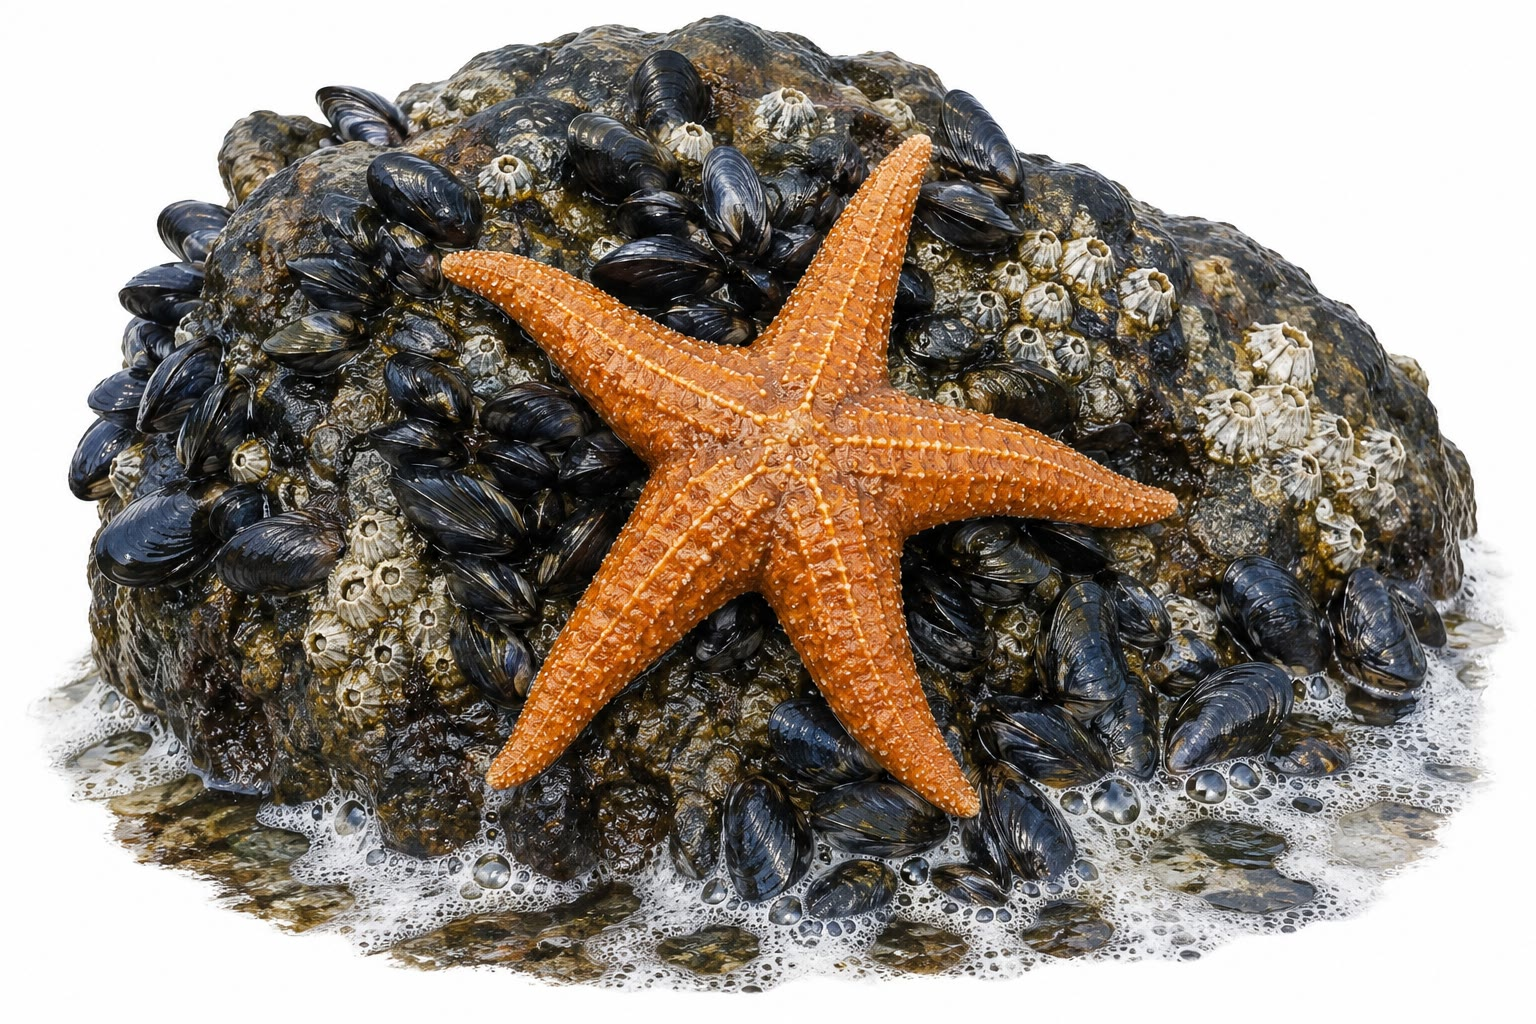
\includegraphics[width=0.6\linewidth]{images/book3/ai/b3-27-sea-star-mussels.jpg}

{\small 低潮时贻贝床上的一只\omterm{def:b1:species-interactions:types}{捕食}性海星：这一关键\omterm{def:b1:species-interactions:types}{捕食}者
一旦被移除，便会使一个原本有十五个物种的海岸
变成贻贝单优\omterm{def:b1:ecosystem-organization:ecosystem}{群落}。}
\end{omfigure}

\section{共同生活：寄生、互利共生、偏利共生}

\begin{definition}[寄生、共生与互利共生]\label{def:b1:species-interactions:symbiosis}
\index{共生}\index{寄生生物}\index{地衣}
\emph{\omterm{def:b1:species-interactions:types}{寄生}生物}生活于宿主之上或之内，
以宿主为代价：体外\omterm{def:b1:species-interactions:types}{寄生}者（如蜱、虱、槲\omterm{def:b1:species-interactions:types}{寄生}）
附着于宿主体表，体内\omterm{def:b1:species-interactions:types}{寄生}者（如绦虫、疟原虫、锈菌）
生活于宿主体内，摄取营养并降低其适合度，
但未必致宿主死亡；\omterm{def:b1:species-interactions:types}{寄生}生物常具专一性，
且常有经由多个宿主的复杂生命周期。\emph{共生}是指两个物种
之间任何紧密而持久的联系；\emph{\omterm{def:b1:species-interactions:types}{互利共生}}则是使双方受益的共生：
\omterm{def:b1:plant-water-minerals:mycorrhiza}{菌根}（真菌附着于或侵入植物根部，
以磷酸盐和水换取\omterm{def:b1:carbohydrates:monosaccharide}{糖类}；见\cref{ch:b1:plant-water-minerals}）、
\omterm{def:b1:plant-water-minerals:nodules}{根瘤}（\omterm{def:b1:plant-water-minerals:nodules}{固氮}细菌由豆科植物供养）、\emph{地衣}（真菌容纳藻类或蓝细菌）、
造礁珊瑚（刺胞动物，容纳进行光合作用的甲藻）、
反刍动物或白蚁的肠道微生物群
（见\cref{ch:b1:digestion-absorption}），以及传粉（花蜜换取花粉的搬运）。
许多\omterm{def:b1:species-interactions:types}{互利共生}起源于\omterm{def:b1:species-interactions:types}{寄生}或\omterm{def:b1:species-interactions:types}{捕食}，
经双方协同演化转为互利，但它们仍是有条件的：
在磷酸盐丰富的土壤中，\omterm{def:b1:plant-water-minerals:mycorrhiza}{菌根}真菌对植物是一种负担，
植物会减少这种联系。
\end{definition}

\begin{example}[传粉：一场交易]\label{ex:b1:species-interactions:pollination}
花朵以数焦耳的糖分制造花蜜；
蜜蜂为采集花蜜而飞行，途中在花朵之间搬运花粉。
花的颜色、气味、形状和开放时间都是针对其传粉者的，
而蜜蜂的舌长、颜色视觉和觅食记忆则针对其花朵；
有些配对紧密契合——例如长花距与唯一能伸及花蜜的蛾类口器——
以至于任何一方离开另一方都无法存活，
整个植物\omterm{def:b1:ecosystem-organization:ecosystem}{群落}甚至可能
依赖少数几种昆虫。
\end{example}

\begin{omfigure}
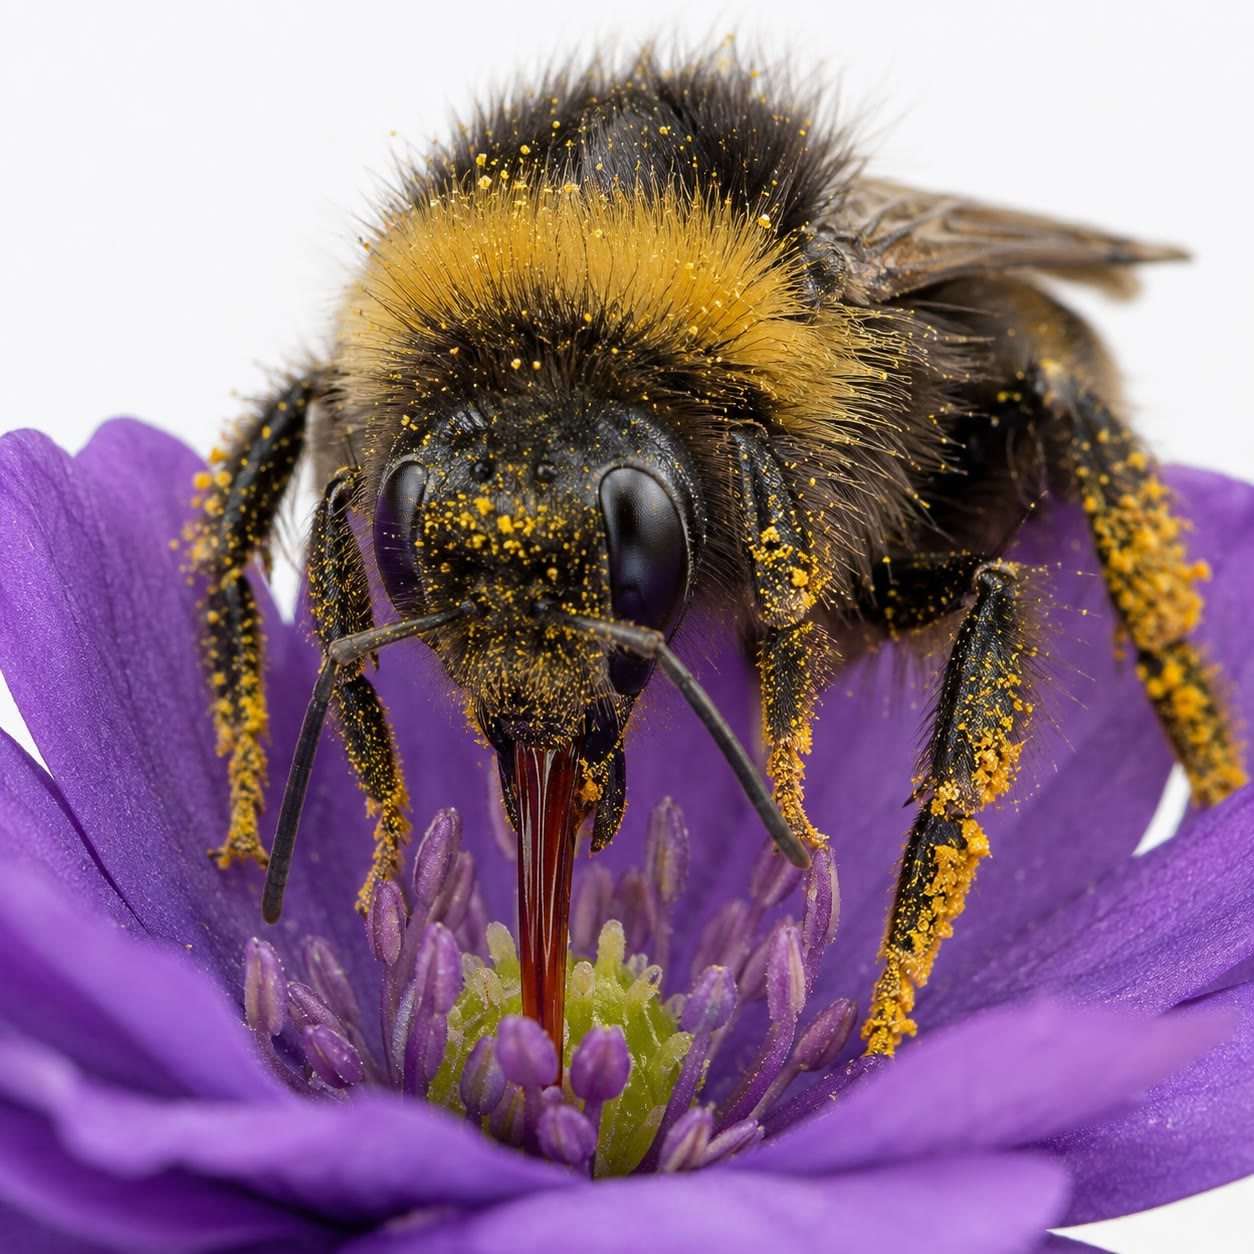
\includegraphics[width=0.56\linewidth]{images/book3/ai/b3-27-bee-flower.jpg}

{\small 正在运作的\omterm{def:b1:species-interactions:types}{互利共生}：蜜蜂获得花蜜，花朵获得花粉的搬运，
双方的形态都经对方塑造。}
\end{omfigure}

\begin{remark}[偏利共生罕见且不稳定]\label{rem:b1:species-interactions:commensal}
真正属于 $+/0$ 的相互作用很少见：遮蔽宿主的附生植物、
使鲨鱼稍受阻力的吸盘鱼、
吃被牛群搅动出的食物的牛背鹭，只在测量精度范围内才可称为\omterm{def:b1:species-interactions:types}{偏利共生}。
相互作用依其净效应分类，
而净效应可能随条件而改变。
\end{remark}

\section{塑造群落的相互作用}

\begin{definition}[关键种、营养级联]\label{def:b1:species-interactions:keystone}
\index{关键种}\index{营养级联}
\emph{关键种}是指其对\omterm{def:b1:ecosystem-organization:ecosystem}{群落}的效应与其丰度
或生物量不成比例的物种：移除它，\omterm{def:b1:ecosystem-organization:ecosystem}{群落}结构便会改变，
通常是因为它控制着一个占优势的\omterm{def:b1:species-interactions:types}{竞争}者。
\emph{\omterm{def:b1:ecosystem-organization:trophic}{营养级}联}是指效应沿\omterm{def:b1:ecosystem-organization:foodweb}{食物链}向下传递，
跨越一个以上\omterm{def:b1:ecosystem-organization:trophic}{营养级}：\omterm{def:b1:species-interactions:types}{捕食}者的存在使植食动物减少，
进而使植物增多；移除\omterm{def:b1:species-interactions:types}{捕食}者则产生相反的效果。
级联表明，\omterm{def:b1:ecosystem-organization:ecosystem}{群落}既受自上而下的\omterm{def:b1:body-plans-tissues:tissue}{组织}，
也受自下而上的\omterm{def:b1:body-plans-tissues:tissue}{组织}（由生产力决定，见\cref{ch:b1:ecosystem-organization}）。
\end{definition}

\begin{proposition}[捕食者可维持多样性]\label{prop:b1:species-interactions:paine}
通过\omterm{def:b1:species-interactions:types}{捕食}那些本会在争夺空间或资源的\omterm{def:b1:species-interactions:types}{竞争}中获胜的物种，
\omterm{def:b1:species-interactions:types}{捕食}者使失败者留在\omterm{def:b1:ecosystem-organization:ecosystem}{群落}中；
移除\omterm{def:b1:species-interactions:types}{捕食}者，则占优势的\omterm{def:b1:species-interactions:types}{竞争}者会排斥这些失败者，多样性
随之下降。
\end{proposition}
\begin{proof}[证据]
佩恩（1966）在北美太平洋沿岸一段
\qty{8}{m} 长的岩石海岸上移除了海星 \emph{Pisaster}，并将
相邻的一段保留为对照。海星
\omterm{def:b1:species-interactions:types}{捕食}贻贝、藤壶和其他固着动物，尤以贻贝为主。
两年之内，贻贝 \emph{Mytilus} 沿岩石向下蔓延，
几乎占据了全部空间；原先生活在空隙中的藤壶、石鳖、帽贝和
藻类相继消失，对照样地的十五个
物种减少为八个。\omterm{def:b1:species-interactions:types}{捕食}者本身在\omterm{def:b1:ecosystem-organization:ecosystem}{群落}生物量中
所占的份额很小；移除它却改变了一切。
\end{proof}

\begin{omfigure}
\begin{tikzpicture}
\begin{axis}[
  width=0.74\linewidth, height=5.6cm,
  axis x line=bottom, axis y line=left,
  xmin=1963, xmax=1969, ymin=0, ymax=18,
  xlabel={年份}, ylabel={样地上的物种数},
  xlabel style={font=\small}, ylabel style={font=\small},
  tick label style={font=\small}, xtick={1963,1964,1965,1966,1967,1968},
  x tick label style={/pgf/number format/1000 sep=},
  legend style={font=\scriptsize, at={(0.98,0.03)}, anchor=south east, draw=none, fill=none},
  legend cell align=left,
]
\addplot[omDef, very thick, mark=*] coordinates {(1963,15) (1964,15) (1965,14) (1966,15) (1967,15) (1968,15)};
\addlegendentry{对照：海星存在}
\addplot[omThm, very thick, mark=square*] coordinates {(1963,15) (1964,12) (1965,10) (1966,9) (1967,8) (1968,8)};
\addlegendentry{移除海星}
\node[font=\scriptsize, anchor=south west, align=left] at (axis cs:1966.2,10.6) {贻贝占满 \\ 岩石};
\end{axis}
\end{tikzpicture}

{\small 佩恩的移除实验（依其数据绘制）。无\omterm{def:b1:species-interactions:types}{捕食}者的样地上，
物种数五年内减半，
而对照样地保持十五个物种。}
\end{omfigure}

\begin{example}[狼、麋鹿与柳树]\label{ex:b1:species-interactions:wolves}
1920 年代，狼从一座大型山地公园中被灭绝；
园中的麋鹿大量繁殖，沿河啃食柳树和白杨，
直至只剩残桩；需要柳树的海狸数量减少，鸣禽
失去了灌丛。1995 年狼被重新引入后，麋鹿数量
下降，更重要的是，它们避开了河谷低地——那里
对它们来说最易受袭击。柳树重新生长，海狸
回来并筑坝，由此形成的湿地又引来了鱼类、两栖动物和鸟类。
这一级联从食肉动物出发，经植食动物传到植物，
再从植物传到十几种从未与狼相遇的物种——其间
天气、狩猎和其他\omterm{def:b1:species-interactions:types}{捕食}者也有作用，因此狼在
这一变化中所占的份额至今仍有争议。
\end{example}

\begin{omfigure}
\begin{tikzpicture}[font=\footnotesize, >=Stealth, line cap=round,
  lv/.style={draw, thick, rounded corners=3pt, inner sep=4pt, align=center, fill=white, minimum width=2.6cm}]
  \node[lv, fill=omDef!25] (wolf) at (0,4.5) {狼};
  \node[lv, fill=omProp!20] (elk) at (0,2.8) {麋鹿};
  \node[lv, fill=omExo!20] (willow) at (0,1.1) {柳树、白杨};
  \node[lv, fill=omProp!20] (beaver) at (3.8,1.1) {海狸};
  \node[lv, fill=omDef!12] (wet) at (7.4,1.1) {池塘、湿地};
  \node[lv, fill=omThm!15] (birds) at (3.8,-0.6) {鸣禽、鱼类、\\ 两栖动物};
  \draw[->, very thick, omThm] (wolf) -- (elk) node[midway, right] {$-$：减少，并使其远离河岸};
  \draw[->, very thick, omThm] (elk) -- (willow) node[midway, left] {$-$：啃食};
  \draw[->, very thick, omDef] (willow) -- (beaver) node[midway, above=9pt] {$+$：食物、水坝};
  \draw[->, very thick, omDef] (beaver) -- (wet) node[midway, above] {$+$};
  \draw[->, very thick, omDef] (willow) -- (birds) node[midway, below left] {$+$};
  \draw[->, very thick, omDef] (wet) |- (birds) node[pos=0.8, below] {$+$};
  \node[anchor=north, align=center, gray] at (3.4,-1.5) {两个负号得正号：狼的回归增加了柳树，\\ 而柳树又将效应传递给狼从未接触过的物种};
\end{tikzpicture}

{\small \omterm{def:b1:species-interactions:keystone}{营养级联}：效应沿三个\omterm{def:b1:ecosystem-organization:trophic}{营养级}向下传递，并
横向贯穿整个\omterm{def:b1:ecosystem-organization:ecosystem}{群落}。符号给出
各环节的作用方向。}
\end{omfigure}

\begin{omfigure}

\includegraphics[width=0.6\linewidth]{images/book3/ai/b3-27-wolves-elk.jpg}

{\small 冬季河谷中的狼与麋鹿。\omterm{def:b1:species-interactions:types}{捕食}者对植被的
影响，既取决于麋鹿敢于在何处觅食，
也取决于它们的数量多少。}
\end{omfigure}

\begin{method}[由实验读出相互作用]\label{met:b1:species-interactions:reading}
\begin{enumerate}
  \item 确定所施加的操作（移除、添加、隔离笼、
        培养中的配对），以及与之并行保留的对照，
        两者处于相同条件下。
  \item 对每个物种，比较有无该伙伴时的丰度：
        差值的符号即给出该物种上
        相互作用的符号。
  \item 寻找间接效应：某个物种未直接接触被操作的物种却发生了变化，
        说明它处于一条链的末端——
        应找出其中的中间环节。
  \item 检查时间尺度（\omterm{def:b1:species-interactions:types}{竞争}可能需要许多代才能分出结果；
        级联以最慢一级的速率进行）
        以及空间尺度（结果能否推广到样地之外？）。
  \item 在数据允许的情况下拟合模型：\omterm{def:b1:species-interactions:types}{竞争}用逻辑斯蒂曲线和
        \omterm{prop:b1:species-interactions:lotka}{等斜线}，\omterm{def:b1:species-interactions:functional}{功能反应}用\omterm{thm:b1:species-interactions:holling}{圆盘方程}，
        并从线性化的图中读出参数。
\end{enumerate}
\end{method}

\section{练习}

\begin{exercise}[$\star$]\label{exo:b1:species-interactions:1}
对六类相互作用中的每一类，
给出其符号组合及一个例子。
\end{exercise}

\begin{exercise}[$\star$]\label{exo:b1:species-interactions:2}
叙述\omterm{def:b1:species-interactions:competition}{竞争排斥原理}，并说明它为何不禁止
一棵云杉上栖息着五只林莺。
\end{exercise}

\begin{exercise}[$\star$]\label{exo:b1:species-interactions:3}
定义\omterm{def:b1:species-interactions:functional}{处理时间}和攻击率，并
求\omterm{def:b1:species-interactions:functional}{处理时间}为 $h = \qty{30}{min}$ 的\omterm{def:b1:species-interactions:types}{捕食}者的最大取食速率。
\end{exercise}

\begin{exercise}[$\star$]\label{exo:b1:species-interactions:4}
什么是\omterm{def:b1:species-interactions:keystone}{关键种}？为什么\omterm{def:b1:species-interactions:keystone}{关键种}不只是
数量最多的物种？
\end{exercise}

\begin{exercise}[$\star\star$]\label{exo:b1:species-interactions:5}
物种 1 的 $K_1 = 500$，物种 2 的 $K_2 = 400$，且 $\alpha =
0.5$ 和 $\beta = 0.6$。画出\omterm{prop:b1:species-interactions:lotka}{等斜线}并给出结果。
再取 $\alpha = 2$，$\beta = 0.6$，重做上述问题。
\end{exercise}

\begin{exercise}[$\star\star$]\label{exo:b1:species-interactions:6}
某\omterm{def:b1:species-interactions:types}{捕食}者的 $a = \qty{0.2}{m^2/h}$，$h = \qty{0.25}{h}$，
分别遇到密度为 \qty{10}{} 和 \qty{100}{} 每平方米的猎物，
求两种情形下的取食速率，以及
其半饱和的猎物密度。
\end{exercise}

\begin{exercise}[$\star\star$]\label{exo:b1:species-interactions:7}
为什么 III 型反应能在低密度下使猎物\omterm{def:b1:populations:population}{种群}稳定，
而 II 型却不能？
\end{exercise}

\begin{exercise}[$\star\star$]\label{exo:b1:species-interactions:8}
根据高斯的实验，解释为何 \emph{P.~bursaria} 能与
\emph{P.~aurelia} 共存，而 \emph{P.~caudatum} 却不能。造成这一差异的
是增长速率还是\omterm{def:b1:ecosystem-organization:niche}{生态位}？
\end{exercise}

\begin{exercise}[$\star\star$]\label{exo:b1:species-interactions:9}
贝茨拟态者的数量比其有毒的模型物种更多。预测
两者所获得的保护将如何变化，
以及为何拟态者的成功是自我限制的。
\end{exercise}

\begin{exercise}[$\star\star\star$]\label{exo:b1:species-interactions:10}
佩因的移除样地失去了七个物种。请用\omterm{prop:b1:species-interactions:lotka}{等斜线}模型解释，
\omterm{def:b1:species-interactions:types}{捕食}优势\omterm{def:b1:species-interactions:types}{竞争}者的\omterm{def:b1:species-interactions:types}{捕食}者如何把
排斥转化为共存。
\end{exercise}

\begin{exercise}[$\star\star\star$]\label{exo:b1:species-interactions:11}
一种\omterm{def:b1:plant-water-minerals:mycorrhiza}{菌根}真菌获取植物 \qty{15}{\%} 的光合产物，
并提供其 \qty{80}{\%} 的磷酸盐。在何种条件下
二者的关系属于\omterm{def:b1:species-interactions:types}{互利共生}，在何种条件下属于\omterm{def:b1:species-interactions:types}{寄生}？
设计一个实验加以区分。
\end{exercise}

\begin{exercise}[$\star\star\star$]\label{exo:b1:species-interactions:12}
设计一个实验，检验柳树的恢复是狼而非天气
或狩猎所引起的：对照、重复、需测量的变量，
以及何种结果将推翻\omterm{def:b1:species-interactions:keystone}{营养级联}。
\end{exercise}

\section{问题：捕食者与海岸}

\begin{problem}[{周末问题——试管中的高斯纤毛虫，
捕食者取食数据的圆盘方程拟合，佩因的海岸（有、无海星），
传粉者的预算，结束于
捕食者的攻击率与处理时间}]
\label{pb:b1:species-interactions:1}

\medskip
\noindent\textbf{第一部分——试管中的\omterm{def:b1:species-interactions:types}{竞争}。}
两种纤毛虫分别单独培养：物种 A 在每
\qty{0.5}{mL} 中达到 $K_A = 200$，$r_A = \qty{0.8}{d^{-1}}$；物种 B 达到
$K_B = 130$，$r_B = \qty{0.55}{d^{-1}}$。共同培养时，一个 B 个体
所耗食物与 $\alpha = 1.4$ 个 A 相当，而一个 A 个体
则与 $\beta = 0.9$ 个 B 相当。
\begin{enumerate}
  \item 在坐标轴上写出两条\omterm{prop:b1:species-interactions:lotka}{等斜线}及其截距。
  \item 画出它们，指出哪一物种获胜，并说明
        结果为何与初始数量无关。
  \item 由倍增时间（$\ln 2/r$），仅凭增长速率，
        你会预期哪一物种获胜？
  \item 第三个物种 C 以试管底部为食，与 A 仅有较弱\omterm{def:b1:species-interactions:types}{竞争}
        （$\alpha = 0.3$，$\beta = 0.3$，$K_C = 100$）。
        画出\omterm{prop:b1:species-interactions:lotka}{等斜线}并给出结果。
  \item 为何排斥原理在试管中成立，而在森林中
        常常失效？请给出两个理由。
  \item 由\omterm{prop:b1:species-interactions:lotka}{等斜线}的交点计算 A 与 C 的
        平衡数量。
\end{enumerate}

\medskip
\noindent\textbf{第二部分——\omterm{thm:b1:species-interactions:holling}{圆盘方程}。}
一只\omterm{def:b1:species-interactions:types}{捕食}性甲虫面对的猎物密度（每平方米）分别为 5、10、20、40 和
80，其每天分别取食 2.0、3.3、5.0、6.7 和 8.0
个猎物。
\begin{enumerate}[resume]
  \item 画出取食速率随密度变化的图，并判断
        反应的类型。
  \item 计算每个数据点的 $1/f$ 与 $1/N$，并作图。
  \item 由斜率和截距求出 $a$ 与 $h$。
  \item 计算最大取食速率与半饱和
        密度。
  \item 在这五个密度中，甲虫在哪一密度下
        处理猎物的时间超过一半？
  \item 甲虫的猎物按逻辑斯蒂方式增长，其中 $r = \qty{0.1}{d^{-1}}$
        且 $K = 200$。猎物的增长（按每平方米无甲虫计）
        与甲虫的消耗相等时，猎物密度为多少？
        （设每平方米有一只甲虫。）此平衡是否
        对猎物的小幅增加稳定？
  \item 出现了第二种猎物，甲虫处理它的速度
        快一倍。预测在高
        密度下甲虫总摄入量的变化。
\end{enumerate}

\medskip
\noindent\textbf{第三部分——岩岸。}
在佩因的对照样地中，\omterm{def:b1:ecosystem-organization:ecosystem}{群落}有 15 个物种；在移除样地中，
物种数在五年间依次下降为 15、12、10、9、8、8，而
贻贝在岩石上的覆盖度由 \qty{20}{\%} 升至 \qty{85}{\%}。
\begin{enumerate}[resume]
  \item 计算一个有 15 个物种且各物种丰度相等的样地的\omterm{def:b1:ecosystem-organization:diversity}{香农指数}，
        以及一个有 8 个物种的样地的\omterm{def:b1:ecosystem-organization:diversity}{香农指数}，其中贻贝占
        个体数的 \qty{85}{\%}，其余七个物种
        平分剩下的部分。
  \item 多样性下降了多少倍？
  \item 结合相互作用的符号，说明为什么移除一个
        $+/-$ 相互作用（海星对贻贝的\omterm{def:b1:species-interactions:types}{捕食}）会使一个 $-/-$
        相互作用（对岩石的\omterm{def:b1:species-interactions:types}{竞争}）增强。
  \item 海星占样地生物量不到 \qty{1}{\%}。
        为什么生物量不能很好地反映一个物种的重要性？
  \item 预测若海星偏好的猎物是最稀有的物种，
        而非占优势的物种，会出现什么结果。
  \item 提出一种方法，以证实起作用的是海星对贻贝的\omterm{def:b1:species-interactions:types}{捕食}，
        而非海星的其他效应（可采用笼养实验）。
\end{enumerate}

\medskip
\noindent\textbf{第四部分——\omterm{def:b1:species-interactions:types}{互利共生}的收支。}
一只蜜蜂一天访问 1000 朵花，采集到 \qty{40}{mg} 糖；
每朵花在花蜜中提供 \qty{40}{\micro g} 糖，并且平均每次访问
从此前的 3 朵花上获得花粉。植物
将其每日光合产物的 \qty{1}{\%}（每朵花 \qty{4}{mg} 糖）用于花蜜；
蜜蜂飞行的代价是每小时觅食消耗 \qty{0.5}{mg} 糖，
（觅食时长 \qty{8}{h}）。
\begin{enumerate}[resume]
  \item 计算蜜蜂每日糖的净收益及其能量当量，
        以 \qty{16}{kJ/g} 换算。
  \item 计算植物每朵花每日的代价占其光合产物的比例，
        并说明这一代价换来了什么。
  \item 为什么这一相互作用是 $+/+$，
        尽管双方都在利用对方？
  \item 一只花蜜盗贼咬穿花的基部，
        不接触花粉而取走花蜜。给出盗贼与植物之间
        相互作用的符号，并说明其对蜜蜂可能的影响。
  \item 画出植物、蜜蜂、盗贼以及\omterm{def:b1:species-interactions:types}{捕食}盗贼的鸟类的符号图，
        并预测该鸟对植物
        的间接效应。
  \item 给出结论：甲虫的攻击率和\omterm{def:b1:species-interactions:functional}{处理时间}，
        以及其最大取食速率。
\end{enumerate}
\end{problem}
